\section{Kernel methods}
\begin{itemize}
	\item Standard parametric models have either fixed basis functions (like linear regression or linear classification models) or learnable basis functions like in neural networks. The training points are solely used to optimize the parameters $\bm{w}$, and all further predictions are based on these optimal parameters
	\item In contrast, kernel methods keep the training data points and also use them (or a subset) during prediction
	\item The predictions are based on a linear combination of the kernel function evaluated on the training data points:
	$$y(\bm{x}) = \sum\limits_{n=1}^{N} \alpha_n k\left(\bm{x}, \bm{x}'\right)$$
	\item For linear models with fixed basis functions, the kernel is:
	$$k(\bm{x},\bm{x}') = \bm{\phi}(\bm{x})^T\bm{\phi}(\bm{x}')$$
	\item The kernel measures \textit{similarity} between $\bm{x}$ and $\bm{x}'$ in features space defined by $\phi(x)$. Thus, it is symmetric: $$k(\bm{x},\bm{x}')=k(\bm{x}',\bm{x})$$
\end{itemize}
\subsection{Kernelizing linear parametric models}
\begin{itemize}
	\item Many linear parametric model can be re-casted into a ``dual representation'' by using the \textbf{kernel trick}: 
	\begin{itemize}
		\item If we have an algorithm formulated in such a way that the input vector $\bm{x}$ enters only in the form of a scalar product, we can replace the scalar product with some other choice of kernel
	\end{itemize}
	\item For instance, the linear regression model is determined by minimizing the regularized sum-of-squares error function given by:
	$$J(\bm{w}) = \frac{1}{2}\sum\limits_{n=1}^{N} \left\{\bm{w}^T \bm{\phi}\left(\bm{x}_n\right) - t_n \right\} + \frac{\lambda}{2}\bm{w}^T \bm{w}$$
	\item Solving the equation of the derivate being equals to 0, we obtain:
	$$\bm{w} = \left(\bm{\Phi}^T\bm{\Phi} +\lambda \bm{I}_M\right)^{-1}\bm{\Phi}^T\bm{t} = \bm{\Phi}^T\left(\bm{\Phi}\bm{\Phi}^T +\lambda \bm{I}_M\right)^{-1}\bm{t} $$
	\item Here, we can replace the inner product $\bm{\Phi}\bm{\Phi}^T$ by the gram matrix $\bm{K}$ where $K_{ij} = \bm{\phi}(\bm{x}_i)^T\bm{\phi}(\bm{x}_j)$
	\item By defining the dual variable $\bm{\alpha} = \left(\bm{K} +\lambda \bm{I}_M\right)^{-1}\bm{t}$, we get the following equations:
	\begin{equation*}
		\begin{split}
			\bm{w} & =\bm{\Phi}^T \bm{\alpha} = \sum\limits_{n=1}^{N} \alpha_n \bm{\phi}(\bm{x}_n)\\
			y\left(\bm{x}'\right) & = \bm{w}^T \bm{\phi}(\bm{x}') = \sum\limits_{n=1}^{N} \alpha_n \bm{\phi}\left(\bm{x}_n\right)^T \bm{\phi}\left(\bm{x}'\right) = \sum\limits_{n=1}^{N} \alpha_n k\left(\bm{x},\bm{x}'\right)
		\end{split}
	\end{equation*}
	\item Thus, we can express linear regression by a dual representation with kernel methods
	\item \textbf{Benefits} of kernel representation:
	\begin{itemize}
		\item We have no explicit parameters/features anymore, only implicit by the kernel function $k(\bm{x},\bm{x}')$
		\item No need to handpick locations of basis functions 
		\item No increase in number of parameters when using kernel methods as those implicitly map inputs to a higher dimensional space
	\end{itemize}
	\item \textbf{Disadvantages}/\textbf{problems}:
	\begin{itemize}
		\item The computational cost to retrieve $\bm{\alpha}$ is $\mathcal{O}(N^3)$ as $\bm{K}\in\mathbb{R}^{N\times N}$ compared to $\mathcal{O}(M^3)$ for calculating $M$ on the standard way (the cost comes from the inverse)
		\item During prediction, we need $\mathcal{O}(N\cdot M)$ to compute the output for a new point, but would only need $\mathcal{O}(N)$ with the primal parameters $\bm{w}$ $\Rightarrow$ slow prediction for large datasets
	\end{itemize}
\end{itemize}
\subsubsection{Constructing valid kernels}
\begin{itemize}
	\item For a valid kernel, the gram matrix $\bm{K}$ must be positive semi-definite for all possible choices of $\left\{x_n\right\}_{n=1}^{N}$
	\item An equivalent constraint would be that $\bm{z}^T \bm{K} \bm{z} \geq 0$ for all $\bm{z}\in\mathbb{R}^{N}$ or the eigenvalues must all be positive (note that $\bm{K}$ can still contain negative elements)
	\item We can construct a kernel from an explicit set of basis functions when we use the expression $k\left(\bm{x},\bm{x}'\right)=\bm{\phi}^T(\bm{x})\bm{\phi}(\bm{x})$
	\item Further, we can construct new kernels by using other valid kernels and extend them by for example multiplying with a constant (no need to know all variations)
	\item Given a valid kernel function, we can derive its corresponding feature vectors (which can be hard and possible infinite). Therefore, we need to express it in the form of $\bm{\phi}(\bm{x})^T \bm{\phi}(\bm{x}')$ where $\bm{\phi}$ must be the same function applied on different points
	\item For example a polynomial kernel of $M=2$ can be rewritten as:
	\begin{equation*}
		\begin{split}
			k\left(\bm{x},\bm{z}\right) & = \left(1+\bm{x}^T\bm{z}\right)^2 = \left(1 + x_1 z_1 + x_2 z_2\right)^2\\
			& = 1 + 2x_1 z_1 + 2x_1 z_2 + (x_1 z_1)^2 + (x_2 z_2)^2 + 2 x_1 z_1 x_2 z_2\\
			& = \left[1, \sqrt{2}x_1, \sqrt{2}x_2, x_1, x_2, \sqrt{2}x_1 x_2\right] \cdot \left[1, \sqrt{2}z_1, \sqrt{2}z_2, z_1, z_2, \sqrt{2}z_1 z_2\right]^T\\
			& = \bm{\phi}(\bm{x})^T \bm{\phi}(\bm{z})
		\end{split}
	\end{equation*}
	\item Here we see that from a two-dimensional vector, we scaled it up to a 6-dimensional feature vector just from our kernel
	\item Some (popular) kernels:
	\begin{itemize}
		\item Generalized polynomial kernel $k\left(\bm{x}, \bm{x}'\right) = \left(c + \bm{x}^T \bm{x}'\right)^{M}$ (feature vector only contains polynomial to order $M$)
		\item Gaussian kernel with infinite feature dimensionality: $k\left(\bm{x}, \bm{x}'\right) = \exp\left(-\frac{1}{2l^2} ||\bm{x}-\bm{x}'||^2\right)$
		\item Radial basis functions of the form $k\left(\bm{x}, \bm{x}'\right) = k\left(||\bm{x}-\bm{x}'||^2\right)$
	\end{itemize}
\end{itemize}
\subsection{Support Vector Machines}
\begin{itemize}
	\item To overcome the slow prediction problem, support vector machines only uses a subset of the training points on which the kernel function needs to be evaluated (also called kernel methods with \textit{sparse} solutions)
	\item It is a convex optimization problem so that only one single optimum exists
	\item No good probabilistic interpretation (see Gaussian Processes for that)
\end{itemize}
\subsubsection{Maximum Margin Classifier}
\begin{itemize}
	\item Similar to discriminant functions in 3.3
	\item For a linearly separable dataset, the maximum margin is defined as the distance between the decision boundary and the closest training point $\Rightarrow$ most robust and stable for perturbations of the input
	\item The distance of a point to the decision boundary is (as previously) defined by:
	$$r_n = \frac{|y(\bm{x}_n)|}{||w||} = \frac{t_ny(\bm{x}_n)}{||w||}\text{\hspace{2mm} if } \bm{x}_n \text{ correctly classified}$$ 
	\item The margin is defined as the minimum distance of decision boundary to any point:
	$$\min_n \frac{t_n \left(\bm{w}^T\bm{x}_n + b\right)}{||\bm{w}||} $$
	\item As we can easily increase the distance by increasing $\bm{w}$ by a factor $\kappa$ and still get the same minimum ($\min_n \frac{t_n \left(\kappa \bm{w}^T\bm{x}_n + \kappa b\right)}{||\kappa \bm{w}||}$), we restrict the choice by setting $t_n \left(\bm{w}^T\bm{x}_n + b\right) = 1$ for the closest point. 
	\item Thus, for all other points, the following constraint must hold: $t_n \left(\bm{w}^T\bm{x}_n + b\right) \geq 1$
	\item A maximum margin is found by maximizing $\frac{1}{||\bm{w}||}$ (as the upper part of the fraction is fixed to 1)
\end{itemize}
\subsubsection{Optimizing Maximum Margin}
\begin{itemize}
	\item To maximize the margin, we try to minimize $\frac{1}{2}||\bm{w}||^2$ (has same optimum as $\frac{1}{||\bm{w}||}$ but is easier to optimize)
	\item By that, we need to fulfill the constraint $t_n \left(\bm{w}^T\bm{x}_n + b\right) \geq 1$ for all data points
	\item To do that, we use Lagrange multiplier for inequalities
	\begin{itemize}
		\item Given the problem to maximize $f(\bm{x})$ subject to $g(\bm{x})\geq 0$, it is equivalent to optimize:
		$$\max_{\bm{x}} \min_{\mu} L\left(\bm{x},\mu\right) = \max_{\bm{x}} \min_{\mu} f(\bm{x}) + \mu g(\bm{x})$$
		\item Note that if we want to minimize $f(\bm{x})$, it is equivalent to maximizing $-f(\bm{x})$: 
		$$\max_{\bm{x}} \min_{\mu} L\left(\bm{x},\mu\right) = \max_{\bm{x}} \min_{\mu} -f(\bm{x}) + \mu g(\bm{x}) \Rightarrow \min_{\bm{x}} \max_{\mu} L\left(\bm{x},\mu\right) = \min_{\bm{x}} \max_{\mu} f(\bm{x}) - \mu g(\bm{x})$$
		\item We have the following (Karush-Kuhn-Tucker) conditions when optimizing this function:
		$$\mu\geq0, \text{\hspace{5mm}}g(\bm{x})\geq0, \text{\hspace{5mm}}\mu\cdot g(\bm{x}) = 0$$
		\item There are two kinds of solutions:
		\begin{itemize}
			\item If the stationary points lies in the region $g(\bm{x})\geq 0$, we have $\nabla f(\bm{x})=0$ and $\mu=0$
			\item Otherwise, if stationary points lies on the boundary we have $\nabla f(\bm{x})=-\mu \nabla g(\bm{x})$
		\end{itemize}
		\item We can solve the optimization problem by first getting a solution for $\tilde{L}(\mu) = \max_{\bm{x}} L(\bm{x},\mu)$, and then optimizing it with respect to $\mu$: $\max_{\mu}\tilde{L}(\mu)$
	\end{itemize}
	\item When we apply this for our maximum margin classifier, we get the following optimization objective with $N$ Lagrange multipliers $a_n$:
	$$L\left(\bm{w},b,\bm{a}\right) = \frac{1}{2}||\bm{w}||^2 - \sum\limits_{n=1}^{N} a_n \left\{t_n \left(\bm{w}^T \bm{x} + b\right) - 1\right\}$$
	\item First, minimize with respect to the primal variables $\bm{w}$ and $b$:
	\begin{equation*}
		\begin{split}
			\frac{\partial L}{\partial \bm{w}} & = \bm{w}^T - \sum\limits_{n=1}^{N} a_n t_n \bm{x}_n^T = 0\to \bm{w} = \sum\limits_{n=1}^{N}a_n t_n \bm{x}_n^T\\
			\frac{\partial L}{\partial b} & = - \sum\limits_{n=1}^{N} a_n t_n = 0\to \sum\limits_{n=1}^{N} a_n t_n = 0\\
		\end{split}
	\end{equation*}
	\item Eliminating $\bm{w}$ and $b$ gives the dual representation $\tilde{L}(\bm{a})$:
	\begin{equation*}
		\begin{split}
			\tilde{L}(\bm{a}) = \sum\limits_{n=1}^{N} a_n - \frac{1}{2} \sum\limits_{n=1}^{N}\sum\limits_{m=1}^{N} a_n a_m t_n t_m \underbrace{\bm{x}_n^T \bm{x}_m}_{k(\bm{x}_n, \bm{x}_m)}
		\end{split}
	\end{equation*}
	\item For prediction, we use the previously derived result $\bm{w} = \sum_{n=1}^{N}a_n t_n \bm{x}_n^T$ to convert it into a kernel:
	$$y(\bm{x})=\bm{w}^T \bm{x} + b = \sum_{n=1}^{N}a_n t_n k(\bm{x}_n, \bm{x})$$
	\item For every data point, $a_n = 0$ or $t_n y(\bm{x}) = 1$. For all points that have $a_n > 0$ influence the prediction, so called support vectors. They lie on maximum margin hyperplanes 
	\item The bias $b$ can be determined by solving $t_n y(\bm{x}_n) = 1$ for a support vector $x_n$
	\begin{figure}[ht]
		\centering
		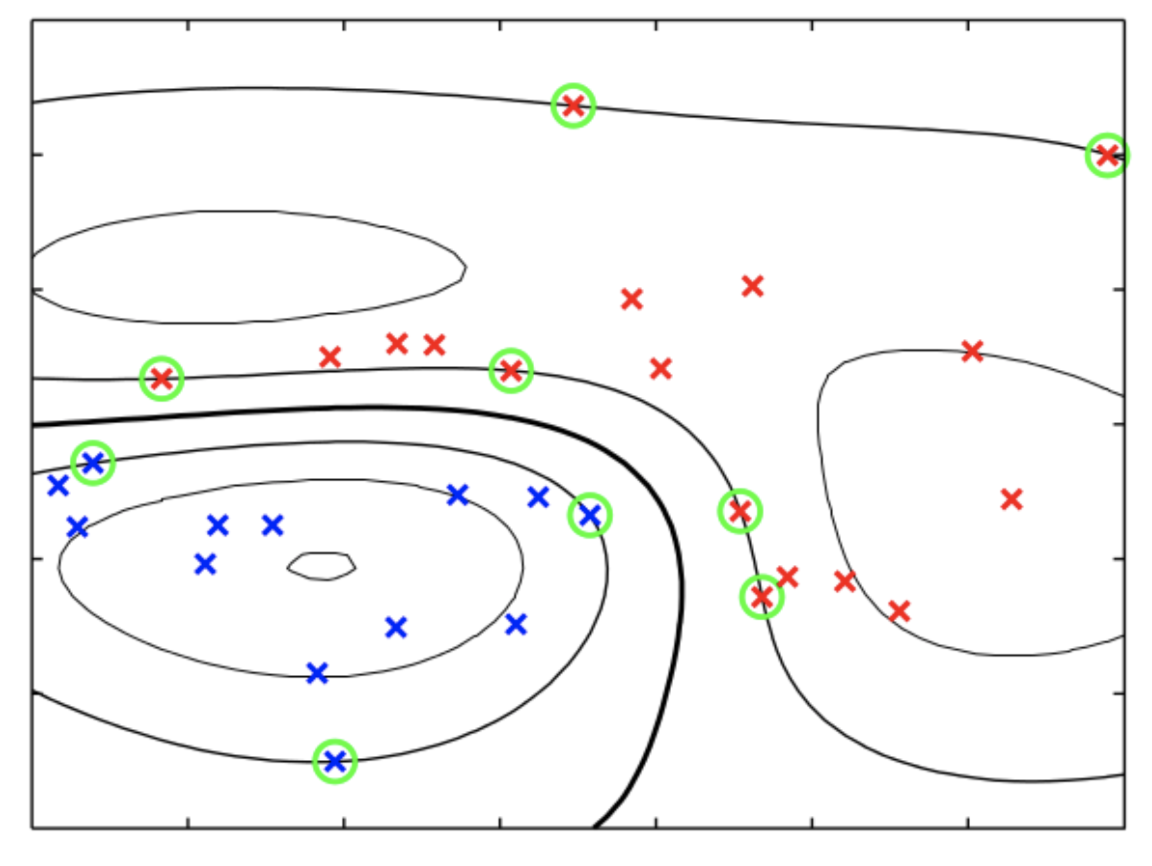
\includegraphics[width=0.3\textwidth]{figures/svm_support_vectors.png}
		\caption{Visualization of non-linear support vectors}
		\label{img:svm_support_vectors}
	\end{figure}
\end{itemize}
\subsubsection{Soft Margin Classifier}
\begin{itemize}
	\item So far we assumed that dataset is (non-linear) separable. However, sometimes distributions overlap 
	\item Thus, soft margin classifier allow data points to be on the "wrong" side of the margin but causing a certain penalty
	\item We introduce \textbf{slack variables} $\xi_n\geq 0$ for $n=1,...,N$
	\item If a point is on the correct side of the margin, its slack variable is $\xi_n = 0$
	\item If it is one the wrong side of the margin, the slack variable is $\xi_n = |t_n - y(\bm{x}_n)|$
	\item Hence, we also have a ``soft'' constraint/margin $t_n y(\bm{x}_n)\geq 1 - \xi_n$
	\begin{figure}[ht]
		\centering
		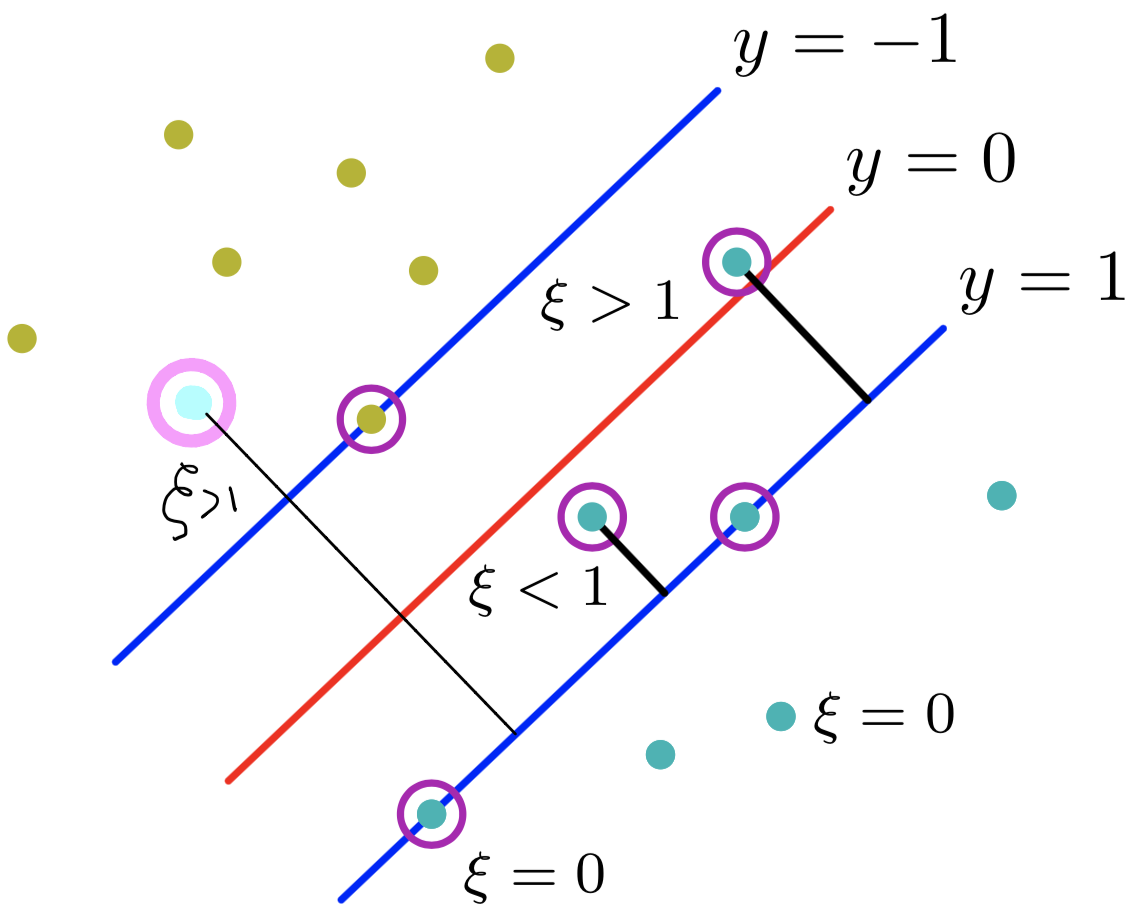
\includegraphics[width=0.3\textwidth]{figures/svm_soft_margin.png}
		\caption{A soft margin classifier uses slack variables to penalize data points on the wrong side.}
		\label{img:svm_soft_margin}
	\end{figure}
	\item The goal is now to maximize the margin while minimizing the penalty given by the slack variables:
	$$\arg\min_{\bm{w},b,\bm{\xi}} \frac{1}{2} ||\bm{w}||^2 + C\sum\limits_{n=1}^{N} \xi_n$$
	\item Introducing the conditions $\xi_n\geq 0$ and $t_n y(\bm{x}_n)\geq 1 - \xi_n$ into the minimization problem, we get the following Lagrangian:
	$$L\left(\bm{w}, b, \bm{\xi}, \bm{a}, \bm{\mu}\right) = \frac{1}{2} ||\bm{w}||^2 +C \sum\limits_{n=1}^{N} \xi_n - \sum\limits_{n=1}^{N} a_n \left\{t_n \left(\bm{w}^T \bm{x}_n + b\right) - 1 + \xi_n \right\} - \sum\limits_{n=1}^{N} \mu_n \xi_n $$
	\item The KKT conditions for the dual variables are:
	\begin{equation*}
		\begin{split}
			& a_n \geq 0,\text{\hspace{3mm}} t_n y(\bm{x}_n) - 1 + \xi_n \geq 0,\text{\hspace{3mm}} a_n \left\{t_n \left(\bm{w}^T \bm{x}_n + b\right) - 1 + \xi_n \right\} = 0\\
			& \mu_n \geq 0,\text{\hspace{3mm}} \xi_n \geq 0,\text{\hspace{3mm}} \mu_n \xi_n = 0\\
		\end{split}
	\end{equation*}
	\item Minimize w.r.t. primal variables $\bm{w}, b, \bm{\xi}$ and use these conditions to eliminate $\bm{w}, b, \bm{\xi}$ from the Lagrangian to obtain the \textbf{dual representation}
	\begin{equation*}
		\begin{split}
			\frac{\partial L}{\partial \bm{w}} & = \bm{w}^T - \sum\limits_{n=1}^{N} a_n t_n \bm{x}_n^T = 0 \implies \bm{w} = \sum\limits_{n=1}^{N} a_n t_n \bm{x}_n\\
			\frac{\partial L}{\partial b} & = - \sum\limits_{n=1}^{N} a_n t_n = 0 \implies \sum\limits_{n=1}^{N} a_n t_n = 0\\
			\frac{\partial L}{\partial \xi_n} & = C - a_n - \mu_n = 0 \implies a_n  = C - \mu_n\\
			\Rightarrow \tilde{L}(\bm{a}) & = \sum\limits_{n=1}^{N} a_n - \frac{1}{2}  \sum\limits_{n=1}^{N}  \sum\limits_{m=1}^{N} a_n a_m t_n t_m \bm{x}_n^T \bm{x}_m
		\end{split}
	\end{equation*}
	\item The remaining constraints are $0\leq a_n \leq C$, and $\sum\limits_{n=1}^{N} a_n t_n = 0$, and we try to \textit{maximize} $\tilde{L}(\bm{a})$
	\item We can also express the dual representation with the kernel trick:
	$$\tilde{L}(\bm{a}) = \sum\limits_{n=1}^{N} a_n - \frac{1}{2}  \sum\limits_{n=1}^{N}  \sum\limits_{m=1}^{N} a_n a_m t_n t_m k(\bm{x}_n, \bm{x}_m)$$
	\item When we want to predict the class for a new test data point $\bm{x}'$, we use:
	$$y(\bm{x}') = \sum\limits_{n=1}^{N} a_n t_n k(\bm{x}_n, \bm{x}') + b$$
	\item Points for different dual parameters:
	\begin{itemize}
		\item Only points with $a_n > 0$ are support vectors and contribute to the prediction
		\item If $C > a_n > 0$, then $t_n y(\bm{x}_n) = 1$ (points on the margin) as $\mu_n > 0$ and hence $\xi_n = 0$
		\item If $a_n = C$, then $\mu_n = 0$ and $\xi_n \geq 0$. When $\xi_n \leq 1$, the points is still correctly classified but within the margin. Otherwise, the point is misclassified
	\end{itemize}
	\item If $C\to\infty$, we recover the hard margin classifier again as we don't allow any outliers
	\item If $C\to 0$, the margin gets really large as we try to maximize the margin without caring about the misclassifications. Also, all points $a_n$ will become support vectors 
\end{itemize}
\subsection{Gaussian Processes}
\subsubsection{Essentials of Gaussian distributions}
\begin{itemize}
	\item \textbf{Marginalization property}: if two random variables $x_1$ and $x_2$ are jointly Gaussian distributed, then marginalizing out one variables still leads to a Gaussian
	$$p\left(\left[\begin{array}{c}
	x_1 \\ x_2
	\end{array}\right]\right) = \left(\left[\begin{array}{c}
	x_1\\x_2
	\end{array}\right]|\left[\begin{array}{c}
	\mu_1\\\mu_2
	\end{array}\right], \left[\begin{array}{cc}
	\Sigma_{11} & \Sigma_{12} \\ \Sigma_{21} & \Sigma_{22} 
	\end{array}\right]\right)\implies\hspace{1mm} p(x_1) = \mathcal{N}(\mu_1, \Sigma_11),\hspace{3mm} p(x_2) = \mathcal{N}(\mu_2, \Sigma_22)$$
	\item \textbf{Conditional property}: if two random variables $x_1$ and $x_2$ are jointly Gaussian distributed, then conditioning one variables on the other still leads to a Gaussian
	$$p(x_1|x_2) = \mathcal{N}(\mu_{1|2}, \Sigma_{1|2})$$
	\item \textbf{Sum property}: Summing two independent Gaussian random variables lead to a new Gaussian variable:
	$$x\sim \mathcal{N}(\mu_1, \Sigma_1) \text{\hspace{1mm}and\hspace{1mm}} y\sim \mathcal{N}(\mu_2, \Sigma_2) \implies x+y=z\sim\mathcal{N}(\mu_1+\mu_2, \Sigma_1+\Sigma_2) $$ 
	\item \textbf{Correlation property}: If $\bm{x}$ is an uncorrelated Gaussian random variable $\mathcal{N}(\bm{0}, \bm{I})$ then $\bm{y} = \bm{\mu} + \bm{A}\bm{x}$ is correlated by $\bm{y}\sim\mathcal{N}(\mu, \bm{A}\bm{A}^T)$
\end{itemize}
\subsubsection{Introduction to Gaussian Processes}
\begin{itemize}
	\item In Bayesian linear regression, we assume that the target is distributed as $t=\bm{\phi}\left(\bm{x}\right)^T \bm{w} + \epsilon$ where $\epsilon\sim\mathcal{N}(0,\beta^{-1})$. The posterior is also Gaussian distributed: $p(\bm{w}|\bm{X},\bm{t}) = \mathcal{N}(\bm{w}|\bm{m}_N, \bm{S}_N)$.
	\item When we predict for new points, we use the mean $\mu_N = \sum_{n=1}^{N}\beta \bm{\phi}(\bm{x})^T \bm{S}_N^{-1} \bm{\phi}(\bm{x}_n)t_n$ % and variance $\sigma_N^2(\bm{x})=\beta^{-1} + \bm{\phi}(\bm{x})^T \bm{S}_N \bm{\phi}(\bm{x})$
	\item Here we see that we can express the mean by the kernel $k(\bm{x}_n, \bm{x}_m) = \bm{\phi}(\bm{x}_n)^T \bm{S}_N^{-1} \bm{\phi}(\bm{x}_m)$ $\Rightarrow$ increase expressiveness of Linear Bayesian regression by using more complex kernels
	\item Definition of Gaussian Processes: A Gaussian process is a collection of random variables, any finite number of which is jointly Gaussian distributed
	\item Gaussian Processes represent distributions over random functions!
	$$f(\circ) \sim \mathcal{N}(m(\circ), k(\circ, \circ))$$
	\item The function \textit{evaluated} at a specific point $\bm{x}$ is a random variable, with $\mathbb{E}[f(\bm{x})] = m(\bm{x})$ and $\text{cov}(f(\bm{x}), f(\bm{x}')) = k(\bm{x}, \bm{x}')$ (covariance matrix is the gram matrix $K$)
	\item Thus, for a finite set of points $\left\{\bm{x}_1, ...,\bm{x}_N\right\}$, the random variables $\left\{f(\bm{x}_1), ...,f(\bm{x}_N)\right\}$ are:
	$$p\left(\begin{bmatrix}
	f(\bm{x}_1)\\
	\vdots\\
	f(\bm{x}_N)\\
	\end{bmatrix}\right) = \mathcal{N}\left(\begin{bmatrix}
	m(\bm{x}_1)\\
	\vdots\\
	m(\bm{x}_N)\\
	\end{bmatrix}, \begin{bmatrix}
	k(\bm{x}_1, \bm{x}_1) & \cdots & k(\bm{x}_1, \bm{x}_N)\\
	\vdots & \ddots & \vdots\\
	k(\bm{x}_N, \bm{x}_1)& \cdots & k(\bm{x}_N, \bm{x}_N)\\
	\end{bmatrix}\right)$$
	\item Each entry is the sampled function evaluated at point $\bm{x}$. We can evaluate/sample functions by just using a fine-grained set of points
	\item The kernel has a significant influence on how the functions might look like. When we consider the kernel $k(\bm{x}_n, \bm{x}_m) = \theta_0 \exp\left(-\frac{1}{2\theta_1}||\bm{x}_n - \bm{x}_m||^2\right) + \theta_2 + \theta_3 \bm{x}_n^T \bm{x}_m$, we see that:
	\begin{itemize}
		\item $\theta_0$ influences the amplitude of the samples of $f$
		\item $\theta_1$ scale the length of correlation
		\item $\theta_2$ introduces a random bias for sampled $f$ (different bias for every sample)
		\item $\theta_3$ adds a linear component into the samples leading to a up-/down-ward trend
	\end{itemize}
\end{itemize}
\subsubsection{Regression with Gaussian Processes}
\begin{itemize}
	\item We have observed data which we model by $f(\bm{x}_i) = y(\bm{x}_i) + \epsilon$ ($\epsilon\sim\mathcal{N}(0,\beta^{-1})$)
	\item We can now model $y$ as GP: 
	$$p\left(\begin{bmatrix}
	y(\bm{x}_1)\\
	\vdots\\
	y(\bm{x}_N)\\
	\end{bmatrix}\right) = \mathcal{N}\left(\bm{0}, \begin{bmatrix}
	k(\bm{x}_1, \bm{x}_1) & \cdots & k(\bm{x}_1, \bm{x}_N)\\
	\vdots & \ddots & \vdots\\
	k(\bm{x}_N, \bm{x}_1)& \cdots & k(\bm{x}_N, \bm{x}_N)\\
	\end{bmatrix}\right)$$
	\item Then, $f(\circ)$ is also a GP since $\bm{f} = \bm{y} + \epsilon$ ($\bm{f}\sim \mathcal{N}(\bm{0}, K(\bm{X}, \bm{X}) + \beta^{-1}\bm{I})$)
	\item For new test data points, we can predict them by using:
	$$p\left(\begin{bmatrix}
	\bm{f}\\
	\bm{f}^{*}\\
	\end{bmatrix}\right) = \mathcal{N}\left(\bm{0}, \begin{bmatrix}
	K(\bm{X}, \bm{X}) + \beta^{-1}\bm{I} & K(\bm{X},\bm{X}^{*})\\
	K(\bm{X}^{*},\bm{X}) & K(\bm{X}^{*}, \bm{X}^{*}) + \beta^{-1}\bm{I}\\
	\end{bmatrix}\right)$$
	\item The more points we see the more certain our predictions gets
	\item Kernel parameters can be chosen based on MLE on training observations
\end{itemize}